\documentclass{article}

% Language setting
% Replace `english' with e.g. `spanish' to change the document language
\usepackage[english]{babel}

% Set page size and margins
% Replace `letterpaper' with `a4paper' for UK/EU standard size
\usepackage[letterpaper,top=2cm,bottom=2cm,left=3cm,right=3cm,marginparwidth=1.75cm]{geometry}

% Useful packages
\usepackage{amsmath}

\usepackage{graphicx}
\usepackage[colorlinks=true, allcolors=blue]{hyperref}

\title{Promove Estatítica - Ozias Filho}
\author{Ingryd França}

\begin{document}


\maketitle

\section{Promove}

    No Promove Estatística realizamos eventos de divulgação do curso de Estatística e da profissão de Estatístico nas escolas de Fortaleza e trazemos profissionais atuantes no mercado de trabalho para falar sobre as experiências deles(as) ou sobre temas importantes para a formação e atuação do Estatístico.

    Nesta Edição tivemos a honra de receber Ozias Filhos, que nos contou sobre sua trajetória acadêmica e experiências no mercado de trabalho, mediádo por Jonas Freire.

    Abaixo está um gráfico mostrando a coleta de dados dos folhetos de feedbacks oferecidos pelo PET, com o objetivo de saber mais sobre a opnião da platéia sobre o evento, palestra e projeto.

\section{Adicionando os valores das Respostas em variáveis.}

- Adicionando os primeiros dados das respostas referente as suas respectivas questões em um data.frame pelo RStudio para melhor construção do gráfico depois.

\subsection{Questão 01}

dados1 = data.frame(

  Resposta = factor(c("Discordo Completamente", "Discordo", "Neutro", "Concordo", "Concordo Completamente"),
  
                    levels = c("Discordo Completamente", "Discordo", "Neutro", "Concordo", 
                               "Concordo Completamente")),
                               
  Quantidade = c(0, 2, 3, 16, 31)
  
)

\subsection{Questão 02}

dados2 = data.frame(

  Resposta = factor(c("Discordo Completamente", "Discordo", "Neutro", "Concordo", "Concordo Completamente"),
  
                    levels = c("Discordo Completamente", "Discordo", "Neutro", "Concordo", 
                               "Concordo Completamente")),
                               
  Quantidade = c(0, 1, 6, 17, 27)
  
)


\subsection{Questão 03}

dados3 = data.frame(

  Resposta = factor(c("Discordo Completamente", "Discordo", "Neutro", "Concordo", "Concordo Completamente"),
  
                    levels = c("Discordo Completamente", "Discordo", "Neutro", "Concordo", 
                               "Concordo Completamente")),
                               
  Quantidade = c(0, 0, 2, 7, 44)
  
)


\subsection{Total}

dadost = data.frame(

  Resposta = factor(c("Discordo Completamente", "Discordo", "Neutro", "Concordo", "Concordo Completamente"),
  
                    levels = c("Discordo Completamente", "Discordo", "Neutro", "Concordo", 
                               "Concordo Completamente")),
                               
  Quantidade = c(0, 3, 11, 40, 102)
  
)




\section{Gráficos}

- Aqui estão os gráficos das respectivas questões do formulário d feedback.

\vspace{1.5cm}


\begin{figure}[htbp]
    \centering
    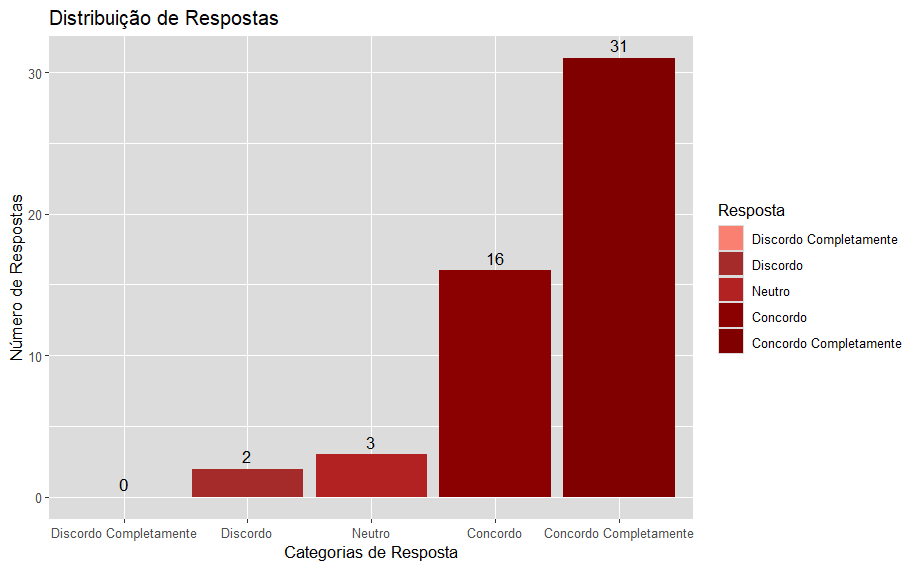
\includegraphics[width=0.8\linewidth]{Rplot_Q1.png}
    \caption{Distribuição de respostas - Questão 01}
    \label{fig:q1}
\end{figure}

\vspace{2\baselineskip}

- O gráfico revela que a maioria dos participantes concordou completamente (31 respostas) que a organização do evento atendeu suas expectativas. Houve ainda 16 respostas na categoria "Concordo", 3 neutras e apenas 2 discordâncias. Essa distribuição apresenta assimetria a esquerda, com a cauda mais alongada à esquerda, indicando predominância de avaliações positivas.


\vspace{1.5cm}
\begin{figure}[htbp]
    \centering
    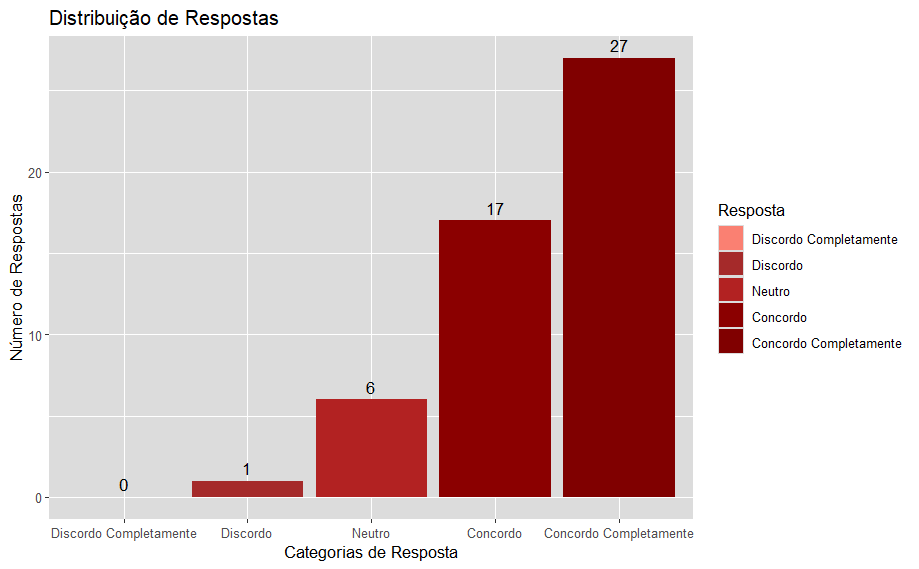
\includegraphics[width=0.8\linewidth]{Rplot_Q2.png}
    \caption{Distribuição de respostas - Questão 02}
    \label{fig:q2}
\end{figure}

\vspace{1cm}

\newpage
- Novamente observamos concentração na resposta "Concordo Completamente" (27 respostas), seguida por "Concordo" (17). Apenas 6 participantes se declararam neutros e 1 discordou da afirmação sobre a contribuição da palestra para o entendimento da carreira estatística. Mantém-se o padrão de assimetria a esquerda, reforçando a tendência de avaliações positivas.

\vspace{1cm}

\begin{figure}[htbp]
    \centering
    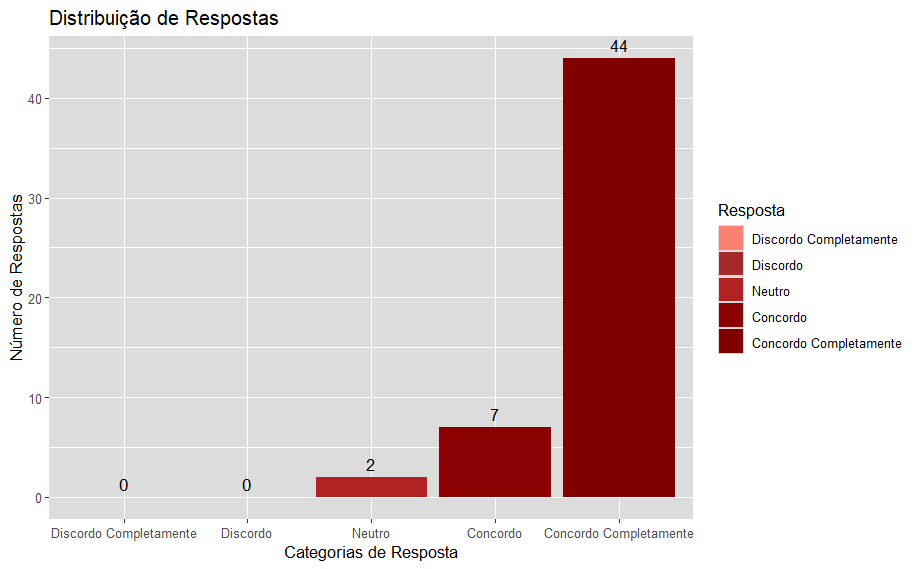
\includegraphics[width=0.8\linewidth]{Rplot_Q3.png}
    \caption{Distribuição de respostas - Questão 03}
    \label{fig:q3}
\end{figure}

\newpage
- Este item apresentou o resultado mais extremo: 44 participantes concordaram completamente que o Promove Estatística efetivamente divulga a profissão, enquanto 7 concordaram e apenas 2 foram neutros. Notavelmente, não houve discordâncias. A forte assimetria a esquerda confirma o reconhecimento quase unânime do projeto.

\vspace{1.7cm}

\begin{figure}[htbp]
    \centering
    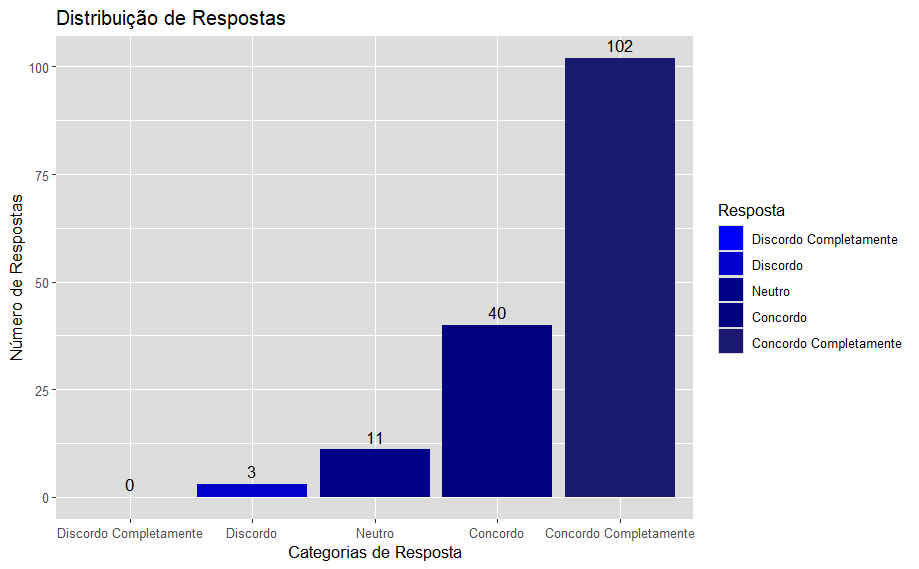
\includegraphics[width=0.8\linewidth]{Rplot_T.png}
    \caption{Distribuição de respostas - Consolidação geral}
    \label{fig:total}
\end{figure}

\vspace{0.5cm}
- O gráfico final no qual leva em considerção todas as perguntas respondidas nos mostra uma recorrência nos casos anteriores com uma distribuição ainda assimétrica a esquerda, a moda permantece em "Concordo Completamente". Sendo eles 102 que concordam completamente, 40 deles apenas concordam, 11 são neutros e 3 discordão, considerando o total respondido de cada item dentre as perguntas.

\section{Conclusão}

Os resultados são tendênciosos para o Concordo Completamente, oque pode sugerir que os dados estão inflados, talvez considerando que os expectadores não responderam de froma sincera. Contudo, vemos a alta frequência de pessoas que marcaram "Concordo Completamente" e "Concordam" na terceira questão, referente ao papel do Promove Estatística na disseminação da Estatítica, nos dando o resultado de que dentre os dados inflados, considerando os gráficos anteriores, o papel do Promove contribui bastante com o entendimento da carreira profissional e acadêmica Estatística.

\section{Códigos}

- Todos os códigos feitos no RStudio utilizando o pacote (ggplot2) para a construção dos gráficos. Antes da criação dos gráficos foi utilizado o comando "library(ggplot2)" para chamar o pacote e utiliza-lo.

\subsection{Gráfico 1}
\newpage

ggplot(dados1, aes(x = Resposta, y = Quantidade, fill = Resposta)) +

  geom-bar(stat = "identity") +
  
  geom-text(aes(label = Quantidade), vjust = -0.5, size = 4) +
  
  labs(
  
    title = "Distribuição de Respostas",
    
    x = "Categorias de Resposta", 
    
    y = "Número de Respostas"
    
  ) +
  
  scale-fill-manual(values = c("FA8072", "A52A2A", "B22222", "8B0000", "800000")) +
  
  theme(panel.background = element-rect(fill = "DCDCDC"))

\subsection{Gráfico 2}

ggplot(dados2, aes(x = Resposta, y = Quantidade, fill = Resposta)) +

  geom-bar(stat = "identity") +
  
  geom-text(aes(label = Quantidade), vjust = -0.5, size = 4) +
  
  labs(
  
    title = "Distribuição de Respostas",
    
    x = "Categorias de Resposta",
    
    y = "Número de Respostas"
    
  ) +
  
  scale-fill-manual(values = c("FA8072", "A52A2A", "B22222", "8B0000", "800000")) +
  
  theme(panel.background = element-rect(fill = "DCDCDC"))

\subsection{Gráfico 3}

ggplot(dados3, aes(x = Resposta, y = Quantidade, fill = Resposta)) +

  geom-bar(stat = "identity") +
  
  geom-text(aes(label = Quantidade), vjust = -0.5, size = 4) +
  
  labs(
  
    title = "Distribuição de Respostas",

    x = "Categorias de Resposta",
    
    y = "Número de Respostas"
    
  ) +
  
  scale-fill-manual(values = c("FA8072", "A52A2A", "B22222", "8B0000", "800000")) +
  
  theme(panel.background = element-rect(fill = "DCDCDC"))

\subsection{Gráfico Total}

ggplot(dadost, aes(x = Resposta, y = Quantidade, fill = Resposta)) +

  geom-bar(stat = "identity") +
  
  geom-text(aes(label = Quantidade), vjust = -0.5, size = 4) +
  
  labs(
  
    title = "Distribuição de Respostas",
    
    x = "Categorias de Resposta",
    
    y = "Número de Respostas"
    
  ) +
  
  scale-fill-manual(values = c("0000FF", "0000CD", "00008B", "000080", "191970")) +
  
  theme(panel.background = element-rect(fill = "DCDCDC"))

\end{document}